%----------------------------------------------------------------------------------------
%    PACKAGES AND THEMES
%----------------------------------------------------------------------------------------

\documentclass[aspectratio=169,xcolor=dvipsnames]{beamer}
\usetheme{SimpleDarkBlue}

\usepackage{hyperref}
\usepackage{graphicx} % Allows including images
\usepackage{booktabs} % Allows the use of \toprule, \midrule and \bottomrule in tables

\usepackage{fontspec}
\usepackage{luatexja}
\usepackage{tikz}
\usepackage{pgfplots}
\pgfplotsset{compat=1.18}

\usepackage{appendixnumberbeamer}

\setmainfont{Alegreya Sans Light}[
  ItalicFont={* Italic},
  BoldFont={Alegreya Sans Medium},
  BoldItalicFont={Alegreya Sans Medium Italic}]
\setsansfont{Alegreya Sans Light}[
  ItalicFont={* Italic},
  BoldFont={Alegreya Sans Medium},
  BoldItalicFont={Alegreya Sans Medium Italic}]

% ------------ %
% beamerbutton %
% ------------ %
\newcommand{\goto}[2]{\hyperlink{#2}{\beamergotobutton{#1}}}
\newcommand{\return}[2]{\hyperlink{#2}{\beamerreturnbutton{#1}}}
\newcommand{\extgoto}[2]{\href{#2}{\beamergotobutton{#1}}}

% % --------------------------- %
% % Section title page with toc %
% % --------------------------- %
% \setbeamertemplate{subsection page}{%
%     \usebeamertemplate*{section page}
% }
% \setbeamertemplate{section in toc}[square]
% \setbeamertemplate{subsection in toc}[square]
% \AtBeginSection[]{
% % \sepframe
% \begin{frame}[noframenumbering]{Outline}
%     % \tableofcontents[currentsection]
%     \tableofcontents[currentsection, currentsubsection]
% \end{frame}
% }
% \AtBeginSubsection[]{
%   \begin{frame}[noframenumbering]{Outline}
%     \tableofcontents[currentsection, currentsubsection]
%   \end{frame}
% }

% ------------------------------------ %
% Section title page with Huge bf text %
% ------------------------------------ %
\AtBeginSection[]{
  \begin{frame}[noframenumbering, plain]
    \Huge{\centerline{\textbf{\insertsection}}}
  \end{frame}
}

%%% automatically add spaces into enumerate and itemize environment
\let\tempone\itemize
\let\temptwo\enditemize
\renewenvironment{itemize}{\tempone\addtolength{\itemsep}{\fill}}{\temptwo}
\let\tempa\enumerate
\let\tempb\endenumerate
\renewenvironment{enumerate}{\tempa\addtolength{\itemsep}{\fill}}{\tempb}

%%=============================================================
%%  FOOTLINE TEMPLATE
%%=============================================================

% % --- Footline depends on onesec option: show only current section or full bar ---
% \if@Optiononesec
% % Minimalist footline: only section name and frame number
% \defbeamertemplate*{footline}{shadow theme}{%
%     \leavevmode\hbox{%
%         \hypersetup{linkcolor=white,urlcolor=white,citecolor=white}
%         \begin{beamercolorbox}[wd=1.01\paperwidth, ht=2.5ex, dp=1.125ex, leftskip=.3cm plus1fil, rightskip=0.3cm]{author in head/foot}%
%             \insertshorttitle \insertsection \hfill \insertframenumber \ / \ \inserttotalframenumber%
%         \end{beamercolorbox}%
%     }%
% }
% \else
% % Standard footline: section bar and frame number
\defbeamertemplate*{footline}{shadow theme}{%
    \leavevmode\hbox{%
        \hypersetup{linkcolor=white,urlcolor=white,citecolor=white}
        \begin{beamercolorbox}[wd=1.02\paperwidth, ht=2.5ex, dp=1.125ex, leftskip=.3cm plus1fil, rightskip=0.3cm]{author in head/foot}%
            \insertsectionnavigationhorizontal{.80\textwidth}{}{} \hspace{.3cm} \hfill \#\ \insertframenumber \ / \ \inserttotalframenumber%
        \end{beamercolorbox}%
    }%
}
% \fi

% --- Activate the custom footline ---
\setbeamertemplate{footline}[shadow theme]


%----------------------------------------------------------------------------------------
%    TITLE PAGE
%----------------------------------------------------------------------------------------

% \title[]{}
% \author{ Hui-Jun Chen\inst{1}
% \and Min Fang\inst{2}
% \and Po-Hsuan Hsu\inst{1}
% \and Chi-Yang Tsou\inst{3}
% \institute[]{
%     \inst{1} National Tsing Hua University \and
%     \inst{2} University of Florida \and
%     \inst{3} University of Manchester \and
%     }\vspace{2pt}
% \date{\today} % Date, can be changed to a custom date



\title[Lecture 5]{Graduate Macro Sequence:\\ Two-Side Labor Search Model}
\author[Hui-Jun Chen]{Hui-Jun Chen}
\institute[]{National Tsing Hua University\\ Department of Economics}
\date{\today}

%----------------------------------------------------------------------------------------
%    PRESENTATION SLIDES
%----------------------------------------------------------------------------------------

\begin{document}

% \setbeamercovered{transparent}
%------------------------------------------------
\begin{frame}[plain,noframenumbering]
    % Print the title page as the first slide
    \titlepage
\end{frame}

%%========================================================================================
%\section{Two-Sided Labor Search}
%\label{sec:TwoSided_Search}
%%========================================================================================

%------------------------------------------------
\begin{frame}{Two-sided search [Mortensen (1982), Pissarides (1985)]}
\label{slide:MP_25_Intro}
\small
\begin{itemize}
    \item Two-sided search: unemployed workers seek jobs and firms with unfilled positions seek workers.
    \item A CRS matching function transforms measures of unemployment \(u\) and vacancies \(v\) into new matches \(M(u,v)\).
    \item When a worker and a firm meet, they bargain over the wage \(w\), splitting the \textbf{match surplus}.
    \item Either party can walk away \(\Rightarrow\) outside options matter (threat points).
    \item \textbf{Search externality:} agents ignore how their actions affect \emph{labor market tightness} \(\theta\) and thus other agents' transition rates.
    \item Except under a knife-edge \textbf{Hosios condition}, decentralized equilibrium is \textbf{inefficient}.
\end{itemize}
\end{frame}

%------------------------------------------------
\begin{frame}{Preferences and technologies}
\label{slide:MP_26_Primitives}
\small
\begin{itemize}
    \item Unit measure of identical, infinitely-lived, risk-neutral workers:
    \[
        u(w)=w,\qquad u(c)=c,\qquad \beta\in(0,1).
    \]
    \item Continuum of risk-neutral, profit-maximizing managers (firms), same \(\beta\) (stationary equilibrium).
    \item Production: \(y = z h\), where \(h\in\{0,1\}\) indicates whether the manager is matched with a worker.
    \item To post (advertise) a vacancy, an unmatched manager pays a per-period cost \(p>0\).
    \item Free entry by managers implies: expected PDV of a vacancy equals posting cost (zero-profit condition).
    \item Employment and separations:
    \begin{itemize}
        \item Let \(n\) be the employment rate and \(u=1-n\) the unemployment rate.
        \item Job destruction is exogenous at rate \(\delta\in(0,1)\).
        \item Effective discounting for an existing match: \(\beta(1-\delta)\).
    \end{itemize}
\end{itemize}
\end{frame}

% \section{Matching}
% \label{sec:Matching}

%------------------------------------------------
\begin{frame}{More on matching technology}
\label{slide:MP_27_Matching}
\small
\begin{itemize}
    \item Matching function \(M(u,v)\) is CRS, increasing in \(u,v\), concave.
    \item CRS \(\Rightarrow\) represent as:
    \[
        M(u,v)=u\,M\!\left(1,\frac{v}{u}\right)=u\,M(\theta),
        \qquad \theta\equiv \frac{v}{u}\ \text{(market tightness)}.
    \]
    \item Transition probabilities:
    \[
        q(\theta)\equiv \frac{M(u,v)}{v}=\theta^{-1}M(\theta)
        \quad \text{(probability a vacancy is filled)},
    \]
    \[
        f(\theta)\equiv \frac{M(u,v)}{u}=\theta q(\theta)
        \quad \text{(probability an unemployed worker finds a job)}.
    \]
    \item Common CRS concave form: Cobb--Douglas matching
    \[
        M(u,v)=u^{\alpha}v^{1-\alpha}=u\,\theta^{1-\alpha},\qquad \alpha\in(0,1).
    \]
    Then
    \[
        q(\theta)=\theta^{-\alpha},\quad q'(\theta)=-\alpha\theta^{-(\alpha+1)}<0,
    \]
    and
    \[
        f(\theta)=\theta q(\theta)=\theta^{1-\alpha},\qquad
        q(\theta)+\theta q'(\theta)=(1-\alpha)\theta^{-\alpha}>0.
    \]
\end{itemize}
\end{frame}

%------------------------------------------------
\begin{frame}{CRS matching technology and Beveridge curve}
\label{slide:MP_28_BeveridgeDerive}
\small
\begin{itemize}
    \item CRS evidence (Blanchard \& Diamond, 1989): regress \(\ln M(u_t,v_t)\) on \(\ln u_t,\ln v_t\) and test \(\alpha+(1-\alpha)=1\).
    \item In steady state, job creation equals destruction:
    \[
        M(u,v)=\delta(1-u)\qquad \big(\text{since }n=1-u\big).
    \]
    \item Cobb--Douglas case:
    \[
        u^\alpha v^{1-\alpha}-\delta(1-u)=0.
    \]
    Totally differentiate (holding parameters fixed) to get a negative slope:
    \[
        \frac{dv}{du}=-\frac{\alpha \theta^{1-\alpha}+\delta}{(1-\alpha)\theta^{-\alpha}}<0.
    \]
    \item General CRS case \(M(u,v)=uM(\theta)\) also yields \(\frac{dv}{du}<0\)
    (a Beveridge curve is downward sloping).
\end{itemize}
\end{frame}

%------------------------------------------------
\begin{frame}{The Beveridge curve}
\label{slide:MP_29_BeveridgePlot}
\small
\begin{columns}
    \begin{column}{0.7\textwidth}
\begin{figure}
    \centering
    \caption{Shimer 2003 NBER WP}
    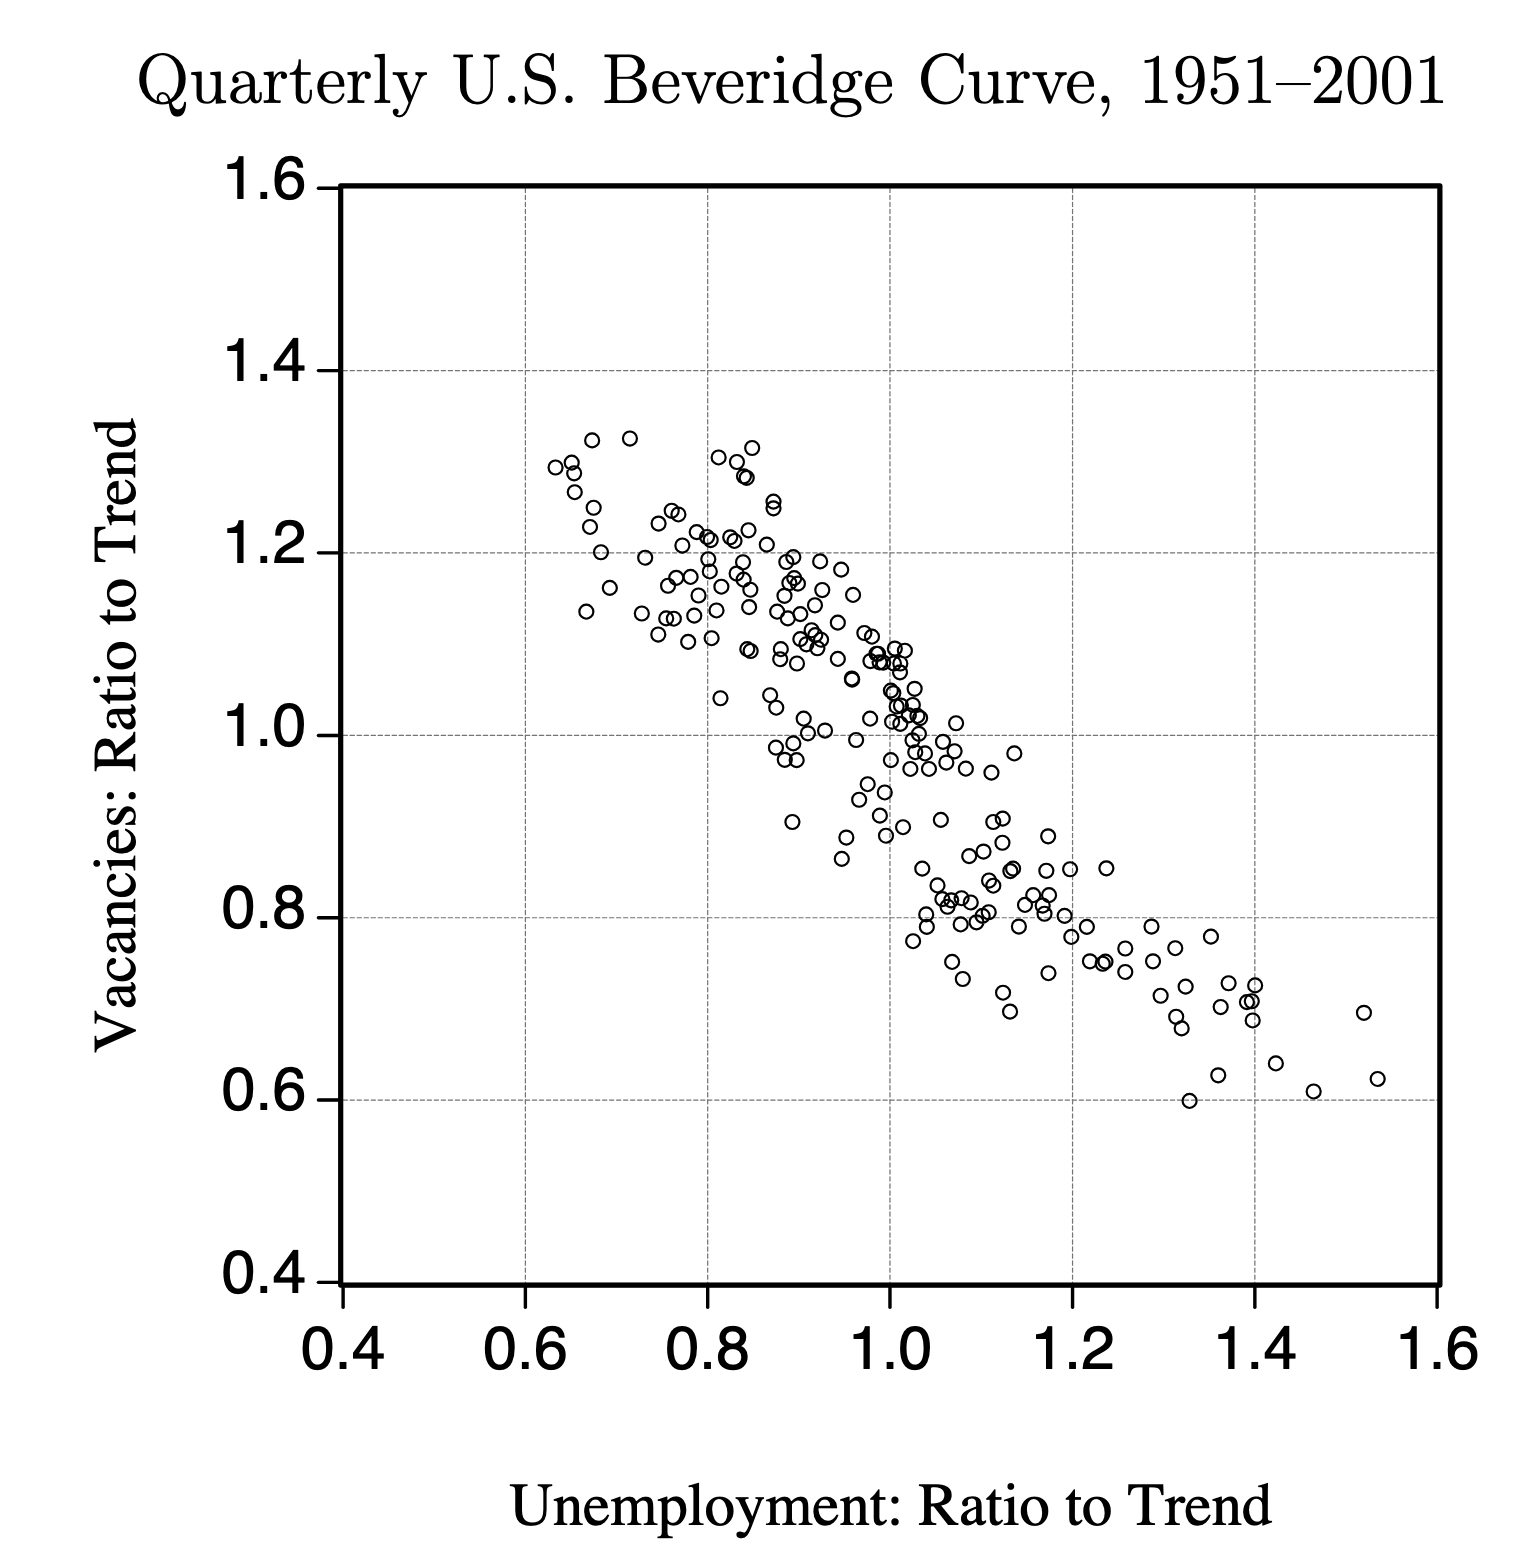
\includegraphics[width=.6\textwidth]{./figures/beveridge.png}
\end{figure}
    \end{column}
    \begin{column}{0.3\textwidth}
        \begin{itemize}
            \item Beveridge curve: negative relation between unemployment \(u\) and vacancies \(v\).
            \item Model-implied slope (C-D):
            \[
                \frac{dv}{du}=-\frac{\alpha \theta^{1-\alpha}+\delta}{(1-\alpha)\theta^{-\alpha}}<0.
            \]
            Similar shape as in aggregate data!
        \end{itemize}
    \end{column}
\end{columns}

% \vspace{0.5em}
% \centering
% \begin{tikzpicture}
% \begin{axis}[
%     width=0.78\linewidth, height=0.45\linewidth,
%     xlabel={$u$ (unemployment)}, ylabel={$v$ (vacancies)},
%     xmin=0, xmax=1, ymin=0, ymax=1,
%     axis lines=left,
%     ticks=none
% ]
% \addplot[smooth, domain=0.08:0.85, samples=100, very thick] ({x},{0.85 - 0.75*x + 0.05*x^2});
% \node[anchor=north east] at (axis cs:0.82,0.30) {Beveridge curve};
% \end{axis}
% \end{tikzpicture}
\end{frame}

%------------------------------------------------
\begin{frame}{Bargaining over match surplus}
\label{slide:MP_30_BargainingIntro}
\small
\begin{itemize}
    \item When a worker and a manager meet, they bargain over wage \(w\).
    \item Worker's Nash bargaining power: \(\phi\in(0,1)\).
    \item Manager's Nash bargaining power: \(1-\phi\).
    \item If bargaining breaks down, they immediately become unmatched.
    \item Off-equilibrium threat points:
    \begin{itemize}
        \item Worker threatens with outside option \(V_u\).
        \item Manager threatens with outside option \(J_u\).
    \end{itemize}
\end{itemize}
\end{frame}

%------------------------------------------------
\begin{frame}{Key equations and definitions so far}
\label{slide:MP_31_SummaryDefs}
\small
\begin{itemize}
    \item Labor market tightness: \(\theta\equiv v/u\).
    \item New matches (hires):
    \[
        M(u,v)=u^\alpha v^{1-\alpha}=u\theta^{1-\alpha}
        \qquad \text{(or }M(u,v)=uM(\theta)\text{)}.
        \tag{1}
    \]
    \item Transition probabilities (manager and worker):
    \[
        q(\theta)\equiv \frac{M(u,v)}{v}=\theta^{-1}M(\theta)\quad (\text{vacancy filling}).
        \tag{2}
    \]
    \[
        f(\theta)\equiv \frac{M(u,v)}{u}=\theta q(\theta)\quad (\text{job finding}).
        \tag{3}
    \]
    \item Worker's bargaining power: \(\phi\).
\end{itemize}
\end{frame}

% \section{Equilibrium}
% \label{sec:Equilibrium}


%------------------------------------------------
\begin{frame}{Decentralized equilibrium: necessary conditions}
\label{slide:MP_32_ValueEqns1}
\small
\textbf{Value of an unemployed worker:}
\[
V_u = c + \beta\Big(f(\theta)V_e + [1-f(\theta)]V_u\Big).
\tag{4}
\]

\textbf{Value of an employed worker:}
\[
V_e = w + \beta\Big(\delta V_u + [1-\delta]V_e\Big).
\tag{5}
\]

\textbf{Value of an unmatched manager (posting a vacancy):}
\[
J_u = -p + \beta\Big(q(\theta)J_e + [1-q(\theta)]J_u\Big).
\tag{6}
\]

\textbf{Value of a matched manager:}
\[
J_e = z-w + \beta\Big(\delta J_u + [1-\delta]J_e\Big).
\tag{7}
\]
\end{frame}

%------------------------------------------------
\begin{frame}{Decentralized equilibrium: free entry}
\label{slide:MP_33_FreeEntry}
\small
Repeat key value equations (workers + managers) and add free entry:

\[
V_u = c + \beta\Big(f(\theta)V_e + [1-f(\theta)]V_u\Big),\tag{4}
\]
\[
V_e = w + \beta\Big(\delta V_u + [1-\delta]V_e\Big),\tag{5}
\]
\[
J_u = -p + \beta\Big(q(\theta)J_e + [1-q(\theta)]J_u\Big),\tag{6}
\]
\[
J_e = z-w + \beta\Big(\delta J_u + [1-\delta]J_e\Big).\tag{7}
\]

\textbf{Free entry of managers:}
\[
J_u=0.
\tag{8}
\]
Plugging \(J_u=0\) into (6) gives the posting-fee relation:
\[
p=\beta q(\theta)J_e.
\tag{9}
\]
\end{frame}

%------------------------------------------------
\begin{frame}{Decentralized equilibrium: unemployment evolution}
\label{slide:MP_34_Bathtub}
\small
With \(u=1-n\), unemployment next period satisfies:
\[
u' = \delta(1-u) + [1-f(\theta)]u.
\tag{10}
\]
Interpretation: next period unemployed are (i) newly separated workers plus (ii) unemployed who fail to find jobs.

\vspace{0.5em}
\textbf{Steady state (bathtub condition):}
\[
\delta(1-u)=u f(\theta)=u\,\theta q(\theta).
\]
So the steady-state unemployment rate is
\[
u=\frac{\delta}{\delta+\theta q(\theta)}.
\tag{11}
\]
\end{frame}

%------------------------------------------------
\begin{frame}{Nash bargaining problem 1 (pie splitting)}
\label{slide:MP_35_Nash1}
\small
\begin{itemize}
    \item Match surplus:
    \[
        S = s_v + s_j = (V_e-V_u) + (J_e-J_u).
    \]
    \item Worker outside option: \(V_u\). Manager outside option: \(J_u=0\).
\end{itemize}

\vspace{0.4em}
\textbf{Nash bargaining (version 1):}
\[
\max_{s_v\in[0,S]} \; s_v^{\phi}(S-s_v)^{1-\phi}.
\]
FOC implies:
\[
\phi(S-s_v)=(1-\phi)s_v
\quad\Rightarrow\quad
s_v=\phi S,\qquad s_j=(1-\phi)S.
\]

\medskip
\textbf{Interpretation:} bargaining splits total surplus in shares \(\phi\) and \(1-\phi\).
\end{frame}

%------------------------------------------------
\begin{frame}{Nash problem and stationary equilibrium defined}
\label{slide:MP_36_Nash2_DefEqm}
\small
\textbf{Nash bargaining (version 2):}
\[
\max_{w}\; (V_e-V_u)^{\phi}(J_e-J_u)^{1-\phi}
\tag{12}
\]
subject to participation constraints:
\[
V_e-V_u\ge 0,\qquad J_e-J_u\ge 0.
\tag{13}
\]

The same pie-sharing condition can be written as:
\[
(V_e-V_u)=\phi S,\qquad (J_e-J_u)=(1-\phi)S,\qquad S=(V_e-V_u)+(J_e-J_u).
\]

\vspace{0.4em}
\textbf{Steady-state equilibrium objects:}
\[
\{V_u,V_e,J_u,J_e,\theta,u,w\}
\]
satisfying (4),(5),(7),(8),(9),(11) and the Nash FOC.
\end{frame}

%------------------------------------------------
\begin{frame}{Determining worker match surplus}
\label{slide:MP_37_WorkerSurplus}
\small
From worker value equation (5):
\[
V_e = w + \beta\Big(\delta V_u + (1-\delta)V_e\Big).
\]
Rearrange in terms of the worker surplus \(V_e-V_u\):
\[
V_e - V_u
= w - (1-\beta)V_u + \beta(1-\delta)(V_e-V_u).
\]
Thus
\[
V_e - V_u
=
\frac{w-(1-\beta)V_u}{1-\beta(1-\delta)}.
\tag{14}
\]
\end{frame}

%------------------------------------------------
\begin{frame}{Determining manager match surplus}
\label{slide:MP_38_ManagerSurplus}
\small
With free entry \(J_u=0\), the matched manager value (7) becomes:
\[
J_e = z-w + \beta(1-\delta)J_e
\quad\Rightarrow\quad
J_e=\frac{z-w}{1-\beta(1-\delta)}.
\tag{16}
\]

\begin{itemize}
    \item (16) implies \(w<z\) is required for \(J_e\ge 0\).
    \item \(V_u\) does not depend on \(w\) directly, but it depends on \(\theta\), which depends on equilibrium.
    \item Sensitivity of worker surplus to \(w\):
    \[
        \frac{\partial (V_e-V_u)}{\partial w}=\frac{1}{1-\beta(1-\delta)}.
    \]
\end{itemize}
\end{frame}

%------------------------------------------------
\begin{frame}{Interior solution to Nash bargaining}
\label{slide:MP_39_NashFOC}
\small
Nash problem:
\[
\max_{w}\; (V_e-V_u)^{\phi}(J_e)^{1-\phi}.
\tag{12}
\]
FOC (using \(\partial(V_e-V_u)/\partial w = 1/[1-\beta(1-\delta)]\) and \(\partial J_e/\partial w=-1/[1-\beta(1-\delta)]\)):
\[
\phi\frac{1}{V_e-V_u}\frac{1}{1-\beta(1-\delta)}
\;+\;
(1-\phi)\frac{1}{J_e}\left(-\frac{1}{1-\beta(1-\delta)}\right)=0.
\]
This simplifies to the key surplus-sharing condition:
\[
(1-\phi)(V_e-V_u)=\phi J_e.
\tag{17}
\]
Next: combine (17) with (14) and (16) to derive the wage.
\end{frame}

%------------------------------------------------
\begin{frame}{Equilibrium wage splits per-period surplus}
\label{slide:MP_40_Wage1}
\small
Use (17): \((1-\phi)(V_e-V_u)=\phi J_e\), together with (14) and (16):
\[
V_e-V_u=\frac{w-(1-\beta)V_u}{1-\beta(1-\delta)},
\qquad
J_e=\frac{z-w}{1-\beta(1-\delta)}.
\]
Multiply by \(1-\beta(1-\delta)\) and rearrange:
\[
(1-\phi)\big[w-(1-\beta)V_u\big] = \phi(z-w).
\]
Solve for wage:
\[
w = \phi z + (1-\phi)(1-\beta)V_u.
\tag{18}
\]

\medskip
\textbf{Interpretation:} wage equals worker's outside option plus a \(\phi\)-share of match surplus.
\end{frame}

%------------------------------------------------
\begin{frame}{Wage as function of labor market tightness}
\label{slide:MP_41_WageTheta}
\small
Start from wage (18):
\[
w = \phi z + (1-\phi)(1-\beta)V_u.
\]
From unemployed worker value (4):
\[
(1-\beta)V_u = c + \beta f(\theta)(V_e-V_u).
\]
From Nash condition (17): \((1-\phi)(V_e-V_u)=\phi J_e\).
Using free entry \(p=\beta q(\theta)J_e\) (9), we get:
\[
(1-\beta)V_u
= c + \beta f(\theta)\frac{\phi}{1-\phi}J_e
= c + \frac{\phi}{1-\phi}\,\theta p.
\quad (\dagger)
\]
Plug (\(\dagger\)) into (18):
\[
w = \phi z + (1-\phi)c + \phi\theta p.
\tag{19}
\]
This is the \textbf{first key} \(w(\theta)\) equation.
\end{frame}

%------------------------------------------------
\begin{frame}{Wage comparative statics}
\label{slide:MP_42_WageCS}
\small
From
\[
w = \phi z + (1-\phi)c + \phi\theta p,
\tag{19}
\]
\begin{itemize}
    \item \(\partial w/\partial z>0\) (productivity raises wages)
    \item \(\partial w/\partial c>0\) (better outside option raises wages)
    \item \(\partial w/\partial \theta>0\) (tight markets raise wages)
    \item \(\partial w/\partial \phi>0\) (more worker power raises wages)
    \item Vacancy cost \(p\): direct effect raises \(\phi\theta p\), but equilibrium \(\theta\) may fall when \(p\) rises.
\end{itemize}

\[
dw = \phi(\theta\,dp + p\,d\theta)
\quad\Rightarrow\quad
\frac{dw}{dp}=\phi\theta + \phi p\frac{d\theta}{dp}.
\]
So the sign of \(dw/dp\) depends on how strongly \(\theta\) falls with \(p\).
\end{frame}

%------------------------------------------------
\begin{frame}{Closing the model: solving market tightness}
\label{slide:MP_43_CloseModel}
\small
We have two key equilibrium relationships involving \(\theta\):

\begin{itemize}
    \item From wage equation (19):
    \[
        z-w = (1-\phi)(z-c) - \phi\theta p.
    \]
    \item From matched manager value (16) and free entry (9):
    \[
        J_e=\frac{z-w}{1-\beta(1-\delta)},
        \qquad
        p=\beta q(\theta)J_e
        \Rightarrow
        (z-w)\beta q(\theta)=p\,[1-\beta(1-\delta)].
    \]
\end{itemize}

Substitute \(z-w\) from the first into the second and rearrange to get an implicit equation for \(\theta\):
\[
z-c
=
\frac{1-\beta[(1-\delta)-\phi\theta q(\theta)]}{(1-\phi)\beta q(\theta)}\,p.
\tag{20}
\]
This \(\theta\) ensures zero expected profits for vacancies and Nash bargaining shares.
\end{frame}

%------------------------------------------------
\begin{frame}{Market tightness in decentralized equilibrium}
\label{slide:MP_44_ThetaCS}
\small
\textbf{(A) Tightness is pinned down by (20):}
\[
(z-c)p^{-1}
=
\frac{1-\beta[(1-\delta)-\phi\theta q(\theta)]}{(1-\phi)\beta q(\theta)}.
\]

\textbf{(B) Matching technology properties (CRS, increasing, concave):}
\[
q(\theta)\ \text{falls in }\theta,\qquad
\theta q(\theta)\ \text{rises in }\theta.
\]

\textbf{(C) Wage rises in \(\theta\):} from (19),
\[
w = \phi z + (1-\phi)c + \phi\theta p.
\]

\medskip
\textbf{Comparative statics intuition via (20):}
\begin{itemize}
    \item \(p\uparrow \Rightarrow\) \(\theta\downarrow\) (vacancies are more expensive) \(\Rightarrow\) tends to reduce \(w\).
    \item \(z\uparrow \Rightarrow\) \(\theta\uparrow\) \(\Rightarrow\) wages rise.
    \item \(c\uparrow \Rightarrow\) \(\theta\downarrow\) (workers are pickier / surplus smaller) \(\Rightarrow\) wages may be pulled down via \(\theta\), but \(c\) directly raises wages in (19).
\end{itemize}
\end{frame}

%------------------------------------------------
\begin{frame}{Planner's problem with search frictions}
\label{slide:MP_45_PlannerSeq}
\small
Planner removes strategic behavior (bargaining) and chooses allocation to maximize discounted output plus home production minus vacancy costs,
subject to matching.

\medskip
No uncertainty; aggregates match individual transition probabilities.
Employment evolves as:
\[
n_{t+1} = (1-\delta)n_t + v_t q(\theta_t),
\qquad
\theta_t \equiv \frac{v_t}{1-n_t}.
\]

\textbf{Sequence problem:}
\[
\max_{\{v_t,n_{t+1}\}_{t\ge0}} \sum_{t=0}^{\infty}\beta^t\big[z n_t + c(1-n_t) - p v_t\big]
\tag{22}
\]
s.t.
\[
n_{t+1}\le (1-\delta)n_t + v_t q\!\left(\frac{v_t}{1-n_t}\right).
\tag{23}
\]
\end{frame}

%------------------------------------------------
\begin{frame}{Recursive formulation of planner's problem}
\label{slide:MP_46_PlannerRec}
\small
Let \(W(n)\) be planner value when employment is \(n\). Bellman form:
\[
W(n)=\max_{v,n'}\Big\{
zn + c(1-n) - pv + \beta W(n') + \Omega\big[(1-\delta)n + v q(\tfrac{v}{1-n}) - n'\big]
\Big\}.
\]

FOC w.r.t. \(v\):
\[
-p + \Omega\Big[q(\theta) + \theta q'(\theta)\Big]=0
\quad\Rightarrow\quad
p=\Omega\Big[q(\theta)+\theta q'(\theta)\Big].
\tag{24}
\]

FOC w.r.t. \(n'\):
\[
\Omega = \beta W'(n').
\tag{25}
\]

Benveniste--Scheinkman:
\[
W'(n)= z-c + \Omega\Big[1-\delta + \theta^2 q'(\theta)\Big].
\tag{26}
\]
\end{frame}

%------------------------------------------------
\begin{frame}{Planner's solution}
\label{slide:MP_47_PlannerSol}
\small
Collect key planner equations:
\[
p=\Omega\big[q(\theta)+\theta q'(\theta)\big],
\qquad
\Omega=\beta W'(n'),
\qquad
W'(n)=z-c+\Omega\big[1-\delta+\theta^2 q'(\theta)\big].
\]

In steady state, \(n,\theta,\Omega\) are constant, so combining (25) and (26) gives:
\[
z-c
=
\Omega\frac{1-\beta[1-\delta+\theta^2 q'(\theta)]}{\beta}.
\tag{27}
\]

Combine (24) and (27) to get the planner's implicit condition for \(\theta\):
\[
z-c
=
\frac{p}{q(\theta)+\theta q'(\theta)}\cdot
\frac{1-\beta[1-\delta+\theta^2 q'(\theta)]}{\beta}.
\tag{28}
\]
\end{frame}

%------------------------------------------------
\begin{frame}{Comparison: equilibrium versus planner's solution}
\label{slide:MP_48_Compare}
\small
\textbf{Decentralized equilibrium \(\theta\) solves (20):}
\[
z-c
=
\frac{1-\beta[(1-\delta)-\phi\theta q(\theta)]}{(1-\phi)\beta q(\theta)}\,p.
\tag{20}
\]

\textbf{Planner \(\theta\) solves (28):}
\[
z-c
=
\frac{p}{q(\theta)+\theta q'(\theta)}\cdot
\frac{1-\beta[1-\delta+\theta^2 q'(\theta)]}{\beta}.
\tag{28}
\]

The two coincide (efficiency) when the \textbf{Hosios condition} holds:
\[
\phi = -\frac{\theta q'(\theta)}{q(\theta)}.
\]
(Equivalently, worker bargaining power equals the elasticity of matches w.r.t. unemployment.)
\end{frame}

%------------------------------------------------
\begin{frame}{Interpreting the Hosios condition}
\label{slide:MP_49_HosiosDerive}
\footnotesize
Define the elasticity of matches w.r.t. unemployment:
\[
\eta_{M,u}\equiv \frac{\partial M(u,v)}{\partial u}\cdot \frac{u}{M(u,v)}.
\]
With CRS form \(M(u,v)=uM(\theta)\), \(\theta=v/u\):
\[
\frac{\partial M}{\partial u}
=
M(\theta) + uM'(\theta)\left(-\frac{v}{u^2}\right)
=
M(\theta)-\theta M'(\theta).
\]
Hence
\[
\eta_{M,u}=\frac{M(\theta)-\theta M'(\theta)}{M(\theta)}.
\]
Using \(q(\theta)\equiv M(u,v)/v=\theta^{-1}M(\theta)\Rightarrow M(\theta)=\theta q(\theta)\),
and differentiating \(q(\theta)=\theta^{-1}M(\theta)\) yields
\[
q'(\theta)=\frac{1}{\theta}\left(M'(\theta)-\frac{M(\theta)}{\theta}\right)
\quad\Rightarrow\quad
M'(\theta)-\frac{M(\theta)}{\theta}=\theta q'(\theta).
\]
Substitute into \(\eta_{M,u}\):
\[
\eta_{M,u}=-\frac{\theta q'(\theta)}{q(\theta)}.
\]
Thus Hosios can be written as \(\phi=\eta_{M,u}\).
\end{frame}

%------------------------------------------------
\begin{frame}{Planner's solution with C-D matching function}
\label{slide:MP_50_PlannerCD}
\small
Impose Cobb--Douglas matching, so \(q(\theta)=\theta^{-\alpha}\) and \(q'(\theta)=-\alpha\theta^{-(\alpha+1)}\).

Planner condition (28):
\[
z-c
=
\frac{p}{q(\theta)+\theta q'(\theta)}
\cdot\frac{1-\beta[1-\delta+\theta^2 q'(\theta)]}{\beta}.
\]
Since \(q(\theta)+\theta q'(\theta)=(1-\alpha)\theta^{-\alpha}\) and \(\theta^2 q'(\theta)=-\alpha\theta^{1-\alpha}=-\alpha\theta q(\theta)\),
\[
z-c
=
\frac{1-\beta[1-\delta-\alpha\theta q(\theta)]}{(1-\alpha)\beta q(\theta)}\,p.
\tag{29}
\]

Recall decentralized condition (20):
\[
z-c
=
\frac{1-\beta[(1-\delta)-\phi\theta q(\theta)]}{(1-\phi)\beta q(\theta)}\,p.
\tag{20}
\]
\end{frame}

%------------------------------------------------
\begin{frame}{Planner's solution versus decentralized outcome}
\label{slide:MP_51_PlannerVsDec}
\small
Planner chooses \(\theta\) via:
\[
(z-c)p^{-1}=\frac{1-\beta[1-\delta-\alpha\theta q(\theta)]}{(1-\alpha)\beta q(\theta)}.
\]
Decentralized equilibrium chooses \(\theta\) via:
\[
(z-c)p^{-1}=\frac{1-\beta[(1-\delta)-\phi\theta q(\theta)]}{(1-\phi)\beta q(\theta)}.
\]

\medskip
\textbf{Same outcome only if Hosios condition holds:}
\[
\phi=\alpha\qquad (\text{equivalently } \phi=\eta_{M,u}).
\]

\medskip
\textbf{Interpretation (externality):}
firms do not internalize how posting a vacancy changes \(\theta\) and thus other agents' matching probabilities.

\medskip
\textbf{Direction:}
\begin{itemize}
    \item If \(\phi<\alpha\): too many vacancies posted (\(\theta\) too high).
    \item If \(\phi>\alpha\): too few vacancies posted (\(\theta\) too low).
\end{itemize}
\end{frame}

%------------------------------------------------
\begin{frame}{Alternative interpretation of Hosios condition}
\label{slide:MP_52_HosiosAlt}
\small
Planner implements efficiency by choosing bargaining weights so that private incentives replicate the planner's \(\theta\).

\medskip
When \(\phi\) rises, the RHS of the decentralized \(\theta\)-condition increases, so \(\theta\) must fall to restore equality.

\vspace{0.6em}
\textbf{Note (elasticity):} elasticity of vacancy filling rate w.r.t. vacancies (C-D):
\[
\eta_{q,v}
=
\left(\frac{\partial q(\theta)}{\partial\theta}\cdot \frac{\partial\theta}{\partial v}\right)\frac{v}{q(\theta)}
=
\left(-\alpha\theta^{-\alpha-1}\cdot\frac{1}{u}\right)\frac{v}{\theta^{-\alpha}}
=-\alpha.
\]

\medskip
If \(\alpha\) is large, one extra vacancy has a large negative effect on vacancy-filling rates for all firms.
Planner response: curtail vacancies by allocating less bargaining power to workers (so that private vacancy posting is reduced).
\end{frame}

%------------------------------------------------
\begin{frame}{Search in an RBC model (preview)}
\label{slide:MP_53_RBCPreview}
\small
\begin{itemize}
    \item Search frictions provide an additional propagation mechanism for business cycles.
    \item Merz (1995, JME) embeds DMP search into an RBC framework:
    \begin{itemize}
        \item aggregate productivity shocks move \(z\),
        \item tightness \(\theta\) and unemployment \(u\) respond endogenously,
        \item wages and vacancies co-move with output in ways RBC without search cannot match.
    \end{itemize}
    \item This is the bridge from ``static labor supply'' to ``frictional labor market'' RBC.
\end{itemize}
\end{frame}

\end{document}
